\documentclass[12pt]{article}
\usepackage[letterpaper,left=2.25cm,top=3.0cm,right=2.25cm,bottom=2.0cm, headsep=1.5cm]{geometry}
\usepackage{fancyhdr}
\usepackage[utf8]{inputenc}
\usepackage[T1]{fontenc}
\usepackage[spanish,mexico]{babel}
%\usepackage[letterpaper,margin=2.5cm]{geometry}
\usepackage{setspace}
\usepackage{titlesec}
\usepackage{tocloft}
\usepackage{graphicx}
\usepackage{longtable}

\usepackage[linguistics]{forest}
\usepackage{amssymb, amsmath, amsbsy} % simbolitos


\usepackage{xcolor}
\usepackage{multirow}
\usepackage{listings}
\lstset{
    basicstyle=\ttfamily\small,
    breaklines=true,
    columns=fullflexible,
    frame=single,
    numbers=left,
    numberstyle=\tiny,
    language=Python,
    keywordstyle=\color{blue},
    commentstyle=\color{gray},
    stringstyle=\color{teal},
    showstringspaces=false,
    extendedchars=true,
    inputencoding=utf8,
    literate=
        {á}{{\'a}}1 {é}{{\'e}}1 {í}{{\'i}}1 {ó}{{\'o}}1 {ú}{{\'u}}1
        {Á}{{\'A}}1 {É}{{\'E}}1 {Í}{{\'I}}1 {Ó}{{\'O}}1 {Ú}{{\'U}}1
        {ñ}{{\~n}}1 {Ñ}{{\~N}}1
        {¿}{{?`}}1 {¡}{{!`}}1
}
\usepackage{caption}
\usepackage{subcaption}
%\usepackage{parskip}
\usepackage[skip=12pt plus1pt]{parskip}
\usepackage{pdfpages} % Incluir PDF en documento en LATEX
\usepackage{verbatim} % comentarios
\usepackage{algpseudocode}
\usepackage{algorithm}
\usepackage{pdflscape}
\usepackage{afterpage}
\usepackage{array,booktabs,ragged2e}
\usepackage{rotating}
%\usepackage{hyperref}
\usepackage{wallpaper}
% \newcolumntype{C}[1]{>{\centering\arraybackslash}p{#1}} % Centrar }
\newcolumntype{L}[1]{>{\raggedright\let\newline\\\arraybackslash\hspace{0pt}}m{#1}}
\newcolumntype{C}[1]{>{\centering\let\newline\\\arraybackslash\hspace{0pt}}m{#1}}
\newcolumntype{R}[1]{>{\raggedleft\let\newline\\\arraybackslash\hspace{0pt}}m{#1}}




% Para utilizar el formato de citas IEEE y comentar los dos parrafos siguientes. Ademas de utilizar el comando \cite en vez de \cite
\usepackage[backend=biber,sorting=none]{biblatex}
% Para utilizar el formato APA, sugiero comentar la linea anterior y descomentar las dos proximas lineas. Ademas de utilizar el comando \cite en vez de \cite
%\usepackage[backend=biber,style=apa]{biblatex}
%\DeclareLanguageMapping{english}{american-apa}

\makeatletter
\DefineBibliographyExtras{spanish}{%
  \setcounter{smartand}{1}%
  \let\lbx@finalnamedelim=\lbx@es@smartand
  \let\lbx@finallistdelim=\lbx@es@smartand
}
\renewbibmacro*{name:delim:apa:family-given}[1]{%
  \ifnumgreater{\value{listcount}}{\value{liststart}}
    {\ifboolexpr{
       test {\ifnumless{\value{listcount}}{\value{liststop}}}
       or
       test \ifmorenames
     }
       {\printdelim{multinamedelim}}
       {\lbx@finalnamedelim{#1}}}
    {}}
\makeatother
% Estas lineas permiten romper los hipervinculos muy largos en las referencias!!!!
\setcounter{biburllcpenalty}{7000}
\setcounter{biburlucpenalty}{8000}
\addbibresource{Referencias.bib} % ARCHIVO DE BIBLIOGRAFÍA


\usepackage[bookmarks=true,breaklinks=true,bookmarksopen=false,colorlinks=true,linkcolor=blue]{hyperref}
\usepackage[hyphenbreaks]{breakurl}
\usepackage{pdfpages} % Incluir PDF en documento en LATEX
\setstretch{1.3}

\usepackage{soul}


% CONSTANTES NECESARIAS PARA EL DOCUMENTO ---> MODIFIQUEN A SU CRITERIO
\newcommand{\NombreAlumno}{Eder Omar Zúñiga Zavala}
\soulregister{\NombreAlumno}{1}
% NUNCA PONGAN EL TITULO EN MAYUSCULAS!!
\newcommand{\NombreProyecto}{Honne S.A. de C.V.}
% Noten los \\ para insertar un ENTER del texto en el encabezado. NUNCA PONGAN EL TITULO EN MAYUSCULAS!!
\newcommand{\NombreProyectoheader}{Honne S.A. de C.V.}
\newcommand{\NombreTSU}{Desarrollo de Software Multiplataforma}
\newcommand{\UnidadEconomica}{Honne S.A. de C.V.}
\newcommand{\nasesorempresaria}   {Oscar David Galindo Olvera}
\newcommand{\nasesorinstitucional}{Dr. Said Polanco Martagón}
\newcommand{\Matricula}           {2430206}  %SU MATRICULA
\newcommand{\ncuatrimestre}{Mayo-Agosto 2026}
% ESTA ES LA FECHA EN LA QUE EL ASESOR INSTITUCIONA EVALUA EL INFORME
\newcommand{\fechaAutorizacionInforme}               {31 de Julio de 2026} 
% ESTA ES LA FECHA EN LA QUE EL ASESOR INSTITUCIONA PROGRAMA LA EXPOSCION 
\newcommand{\DiaEvaluacionPesentacion}{12}
\newcommand{\MesEvaluacionPesentacion}{Agosto}
\newcommand{\AnhoEvaluacionPesentacion}{2026}
\newcommand{\fechaPortada}               {\MesEvaluacionPesentacion~de~\AnhoEvaluacionPesentacion}
\newcommand{\HoraEvaluacionPesentacion}{10:00 hrs}

\newcommand{\modalidadEvaluacionPesentacion}{Presencial} % Otras opciones: Virtual
\newcommand{\tipoAulaOficinaEnlacePesentacion}{la Oficina} % Otras opciones: la oficia/el aula/enlace
\newcommand{\AulaEvaluacionOEnlaceMeetPesentacion}{I-XXX69} %otras opciones: si es un elance de meet, rodearlo \url{}

%\newcommand{\modalidadEvaluacionPesentacion}{Virtual} % Otras opciones: Virtual
%\newcommand{\tipoAulaOficinaEnlacePesentacion}{el enlace} % Otras opciones: la oficia/el aula/el enlace
%\newcommand{\AulaEvaluacionOEnlaceMeetPesentacion}{\url{http://www.upvictoria.edu.mx}} %otras opciones: si es un elance de meet, rodearlo \url{}

\newcommand{\ncarrera}            {Ingeniería en Tecnologías de la Información e Innovación Digital}


\fancyhead{} % Clear all header fields
\fancyhead[C]{%
    \begin{tabular}{@{} m{0.2\textwidth} m{0.5\textwidth} m{0.2\textwidth} @{}}
        % Left image
        \includegraphics[height=1.20cm]{UTYP.png}
        &
        % Center text (multiline, centered)
        \centering
        \scriptsize{\NombreProyectoheader}
        %\textbf{University Name} \\ 
        %Department of Something \\ 
        %Course Title
        &
        % Right image
        %\raggedleft
        \includegraphics[height=1.5cm]{LogoUPV_2023.png}
    \end{tabular}
}


%\usepackage{imakeidx}
%\makeindex[title=New Index Title]

%\renewcommand{\contentsname}{Whatever}
%

%\usepackage[english]{babel}

\addto\captionsspanish{% Replace "english" with the language you use
  \renewcommand{\contentsname}%
    {Contenido temático}%
}


\renewcommand\spanishtablename{Tabla}

\begin{document}

% PAGINA 1 - PORTADA
\setcounter{page}{0}
\pagenumbering{roman}
\thispagestyle{empty}




\begin{titlepage}


\vspace*{-2cm}
\begin{center}
\begin{tabular}{cp{6cm}c}
\includegraphics[height=2.25cm]{UTYP.png} & 
& \includegraphics[height=2.25cm]{LogoUPV_2023.png}   \\
\end{tabular} \\[0.5cm]



{\Large \textbf{UNIVERSIDAD POLITÉCNICA DE VICTORIA}}\\[1.0cm]

{\Large \textbf{REPORTE TÉCNICO DE ACTIVIDADES DE ESTADÍA UNIVERSITARIA}}\\[0.75cm]

{\Large EN \MakeUppercase{\NombreProyecto}}\\[1.0cm]

QUE PRESENTA

\textbf{\MakeUppercase{\NombreAlumno}}\\[1.0cm]

EN CUMPLIMIENTO DE LA ESTADÍA TSU EN\\
\textbf{\MakeUppercase{\NombreTSU}}\\[0.75cm]

ASESOR INSTITUCIONAL\\
\textbf{\MakeUppercase{\nasesorinstitucional}}\\[0.5cm]

UNIDAD ECONÓMICA RECEPTORA:\\
\textbf{\MakeUppercase{\UnidadEconomica}}\\[0.5cm]

ASESOR DE LA UNIDAD ECONÓMICA\\
\textbf{\MakeUppercase{\nasesorempresaria}}\\[0.5cm]


\end{center}
\begin{flushright}
Ciudad Victoria, Tamaulipas, \fechaPortada.
\end{flushright}

\end{titlepage}


\newpage
% PAGINA 1 - PORTADA
\setcounter{page}{0}
\pagenumbering{roman}
\pagestyle{empty}
\ULCornerWallPaper{1}{Membrete2023.pdf}
\vspace*{2cm}



\begin{center}
{\Large \textbf{Formato de autorización para exposición de Estadía de}}\\[0.125cm]
{\Large \textbf{Técnico Superior Universitario}}\\[0.25cm]
\end{center}

\noindent
Fecha y lugar en que se emite: \textbf{Ciudad Victoria, Tamaulipas, a \fechaAutorizacionInforme } \\[0.125cm]
Nombre completo del estudiante: \textbf{\NombreAlumno} \\[0.125cm]
Matrícula: \textbf{\Matricula}  \\[0.125cm]
Programa Académico: \textbf{\ncarrera}  \\[0.25cm]

\noindent
Por medio del presente, se le informa que tras realizar su Estadía en la empresa \textbf{\UnidadEconomica}, desarrollando el \textbf{Reporte Técnico de Actividades de Estadía Universitaria}, durante el periodo comprendido \textbf{\ncuatrimestre} logrando una ponderación de \_\_\_\_  (60\% posibles) para el criterio de reporte; por lo tanto, se otorga la oportunidad de exponer el trabajo realizado por medio de un informe ejecutivo programado para el día \textbf{\DiaEvaluacionPesentacion} del mes de \textbf{\MesEvaluacionPesentacion} del año en curso en un horario de \textbf{\HoraEvaluacionPesentacion} en modalidad \textbf{\modalidadEvaluacionPesentacion} en \textbf{\tipoAulaOficinaEnlacePesentacion} \textbf{\AulaEvaluacionOEnlaceMeetPesentacion}.

\vspace{0.25cm}

\noindent
Sin otro particular, se le recomienda estar disponible para iniciar su exposición 10 minutos antes de la indicación oficial.

\vspace{0.5cm}

\begin{center}
\begin{tabular}{p{10cm}}
\multicolumn{1}{c}{Atentamente}   \\
 \\
 \\ \hline
\multicolumn{1}{c}{\nasesorinstitucional}   \\
\multicolumn{1}{c}{Asesor institucional}   \\
\end{tabular}
\end{center}

\clearpage
\ULCornerWallPaper{1}{Membrete2023.pdf}

\vspace*{3cm}

\begin{center}
{\large \textbf{Control sumativo de Estadía para Técnico Superior Universitario}}
\end{center}

\vspace{0.5cm}

\begin{center}
\begin{tabular}{|p{6cm}|p{4cm}|p{4cm}|}
\hline
\textbf{Criterio} & \textbf{Valor / Ponderación} & \textbf{Calificación} \\ \hline
Reporte & 60\% & \\ \hline
Exposición & 40\% & \\ \hline
Calificación final & \multicolumn{2}{c|}{ } \\ \hline
\end{tabular}
\end{center}

\vspace{0.8cm}

%\noindent
%\textbf{Nota:} para completar este documento deberá sustentar su decisión con base en las rúbricas oficiales de la institución diseñadas para cada evaluación.

\begin{center}
\begin{tabular}{|p{10cm}|}
\hline
\multicolumn{1}{|c|}{\textbf{Datos de la evaluación sumativa}}\\
\multicolumn{1}{|c|}{Fecha: \textbf{\DiaEvaluacionPesentacion}  / \textbf{\MesEvaluacionPesentacion} / \textbf{\AnhoEvaluacionPesentacion}} \\ \hline
%\multicolumn{1}{c}{Atentamente}   \\
 \\
 \\ \hline
\multicolumn{1}{c}{\nasesorinstitucional}   \\
\multicolumn{1}{c}{Asesor institucional}   \\
\end{tabular}
\end{center}




%\vspace{1cm}

%\noindent




%\vspace{1.5cm}

%\noindent
%Firma: \hrulefill

%\vspace{1cm}

%\noindent
%Nombre del Asesor institucional: \nasesorinstitucional \hrulefill


\clearpage
\ClearWallPaper
\thispagestyle{fancy}
\addcontentsline{toc}{section}{Agradecimientos}
\section*{Agradecimientos}

Se agradece a \UnidadEconomica\ por la oportunidad de realizar esta Estadía y por el apoyo brindado durante su desarrollo. De manera particular, se agradece al asesor de la unidad económica, \nasesorempresaria, por su guía y disposición a lo largo de las actividades realizadas, así como al asesor institucional, \nasesorinstitucional, por su acompañamiento y retroalimentación en la elaboración de este reporte.

\clearpage
\thispagestyle{fancy}
\addcontentsline{toc}{section}{Resumen}
\section*{Resumen}

El presente reporte documenta las actividades realizadas durante la Estadía Universitaria en \UnidadEconomica, empresa de transformación tecnológica y consultoría cloud, en su Centro de Operación y Excelencia Multicloud (CCoE) ubicado en calle 533 Maratines, Ciudad Victoria, Tamaulipas. La Estadía se llevó a cabo en la Mesa de Servicio de ese centro, área responsable de vigilar la infraestructura en la nube de los clientes de la empresa y de reportar las fallas que se presentan en ella. El objetivo planteado fue apoyar en el uso de las herramientas de monitoreo del área y en sus actividades diarias, para distribuir la carga de trabajo del equipo.

El trabajo se organizó en cuatro frentes. Las alertas activas de AWS se verificaron con las métricas de Amazon CloudWatch, aplicando un umbral de persistencia de 15 minutos para separar los falsos positivos de los incidentes reales. Los registros de las instancias en Google Cloud Platform se revisaron desde la consola de la plataforma, buscando errores acumulados y latencias sostenidas. Las alertas de ServiceNow se atendieron mediante revisión continua de su bandeja. El monitoreo de las soluciones de TIBCO Scribe se hizo al principio a mano y más adelante con un script en Python desarrollado por iniciativa propia, que notifica las fallas a través de un bot de Telegram; como la plataforma no publica documentación de su API, fue necesario recurrir a la ingeniería inversa para replicar las llamadas que hace su propio panel web. De la formación académica, la materia de Redes fue la que más se aplicó, al facilitar la comprensión de los servicios en la nube y del manejo del panel de AWS.

Las 129 alertas de AWS acumuladas quedaron clasificadas en su totalidad. El script de monitoreo sustituyó una revisión manual que ocupaba entre seis y siete minutos cada media hora, lo que representa cerca de 35 horas de trabajo liberadas al mes. Los objetivos planteados se cumplieron; el desarrollo del script fue la aportación principal de la Estadía, y extender esa automatización a las demás herramientas del área queda como oportunidad de mejora.

\clearpage
\thispagestyle{fancy}
\addcontentsline{toc}{section}{Abstract}
%\vspace*{1cm}
\section*{Abstract}

This report describes the work carried out during a university internship (Estadía) at \UnidadEconomica, a technology transformation and cloud consulting firm, in its Multicloud Operations and Excellence Center (CCoE) at calle 533 Maratines, Ciudad Victoria, Tamaulipas. The internship took place in the center's Service Desk, the team in charge of watching over client cloud infrastructure and reporting any failures found in it. The stated goal was to help operate the team's monitoring tools and share its daily workload.

Four lines of work were covered. Active AWS alerts were checked against Amazon CloudWatch metrics, using a fifteen-minute persistence threshold to tell scheduled activity apart from genuine incidents. Instance logs in Google Cloud Platform were reviewed for accumulated errors and sustained latency. ServiceNow alerts were followed continuously, since that platform sends no automatic notifications of its own. TIBCO Scribe solutions were checked by hand at first, and later monitored by a Python script written on the author's own initiative, which reports failures through a Telegram bot. Because the platform publishes no API documentation, the internal calls made by its web panel had to be reverse-engineered. Of the coursework taken at university, the Networking course proved the most useful, as it made the cloud services and the AWS console easier to understand.

All 129 accumulated AWS alerts were classified. The script replaced a manual check that took six to seven minutes every half hour, freeing roughly 35 hours of the team's time per month. The objectives were met, the script being the main contribution of the internship; extending the same automation to the remaining tools is left as an opportunity for improvement.

\clearpage
%\renewcommand{\indexname}{Contenido temático}

\thispagestyle{empty}
\ClearWallPaper
\tableofcontents


\clearpage
\pagenumbering{arabic}
\setcounter{page}{1}
\pagestyle{fancy}

\section{Introducción}
\label{ch:introduccion}
%Contextualización del tema%
En el ámbito de las operaciones tecnológicas corporativas, la gestión eficiente de tareas y la organización visual de la información son fundamentales para garantizar la continuidad de los servicios \cite{manza-diaz_gestion_2025}. En la empresa Honne S.A. de C.V., específicamente dentro de su Centro de Operación y Excelencia Multicloud (CCoE), el equipo lleva a cabo actividades críticas de alta exigencia para clientes a nivel internacional, abarcando desde el soporte técnico y el monitoreo preventivo de infraestructuras (NOC/SOC), hasta la validación de integraciones de software \cite{honne_oficial_2026}. Tradicionalmente, la delegación, asignación y seguimiento de estas responsabilidades se han administrado mediante el uso de un documento en Excel, el cual funciona como un manual operativo y agendario central. Sin embargo, la gestión de entornos tecnológicos complejos a través de hojas de cálculo plantea retos significativos en la interacción diaria de los empleados, lo que hace evidente la necesidad de evolucionar hacia plataformas que prioricen una experiencia de usuario (UX) fluida y un diseño de interfaz (UI) estructurado para soportar altas cargas operativas \cite{gupta_impact_2026}.


%Problema de investigación%
El problema central de esta investigación radica en la ineficiencia y la saturación visual que genera el uso de Microsoft Excel como herramienta principal para la delegación de tareas en el Centro de Operación y Excelencia Multicloud (CCoE) de Honne S.A. de C.V. Actualmente, el personal se enfrenta a una interfaz estática y desorganizada, donde la información crítica —como el filtrado de actividades (Programadas, Internas, Tibco), el calendario de turnos y las notificaciones de ausencias— se encuentra aglomerada y sin diferenciación por perfiles de usuario (Administrador vs. Empleado). Esta falta de organización visual provoca una navegación confusa, vuelve más lentos los procesos diarios y eleva el riesgo de errores humanos en un entorno que exige respuestas rápidas y alta disponibilidad. Por lo tanto, el presente estudio se delimita espacial y poblacionalmente al personal operativo y administrativo del CCoE, buscando dar respuesta a la siguiente interrogante: ¿De qué manera el diseño de una interfaz web estructurada bajo principios de usabilidad (UX/UI) puede resolver la saturación de información y optimizar el seguimiento de las métricas operativas en el entorno corporativo?

%Justificación, Objetivos, Metodología y Estructura (luego lo extiendo)%
El objetivo principal de este proyecto es diseñar una interfaz gráfica intuitiva y centrada en el usuario que reemplace el actual manual en Excel, reduciendo el tiempo de interacción y mejorando la eficiencia del personal del CCoE. Esta propuesta se justifica por la necesidad de mitigar errores humanos y agilizar la visualización de tareas operativas mediante metodologías de diseño UX/UI y arquitectura de la información. A lo largo de este documento se detallan todos los aspectos relevantes de la investigación, abordando desde los objetivos establecidos y la justificación del diseño, hasta la metodología aplicada, los alcances, limitaciones y los resultados obtenidos en la propuesta visual.

\subsection{Antecedentes}
\label{sec:antecedentes}
En los últimos años, la gestión operativa dentro de las organizaciones tecnológicas ha experimentado una transición acelerada, pasando de procesos administrativos manuales a la adopción de plataformas digitales centralizadas. Esta evolución ha permitido a las empresas escalar el alcance de sus servicios, pero al mismo tiempo ha incrementado la complejidad de la información que los empleados deben procesar diariamente para llevar a cabo sus funciones [4].

Históricamente, la organización interna, el seguimiento de tareas y la comunicación de turnos se apoyaba fuertemente en herramientas ofimáticas genéricas, como hojas de cálculo o documentos de texto compartidos. Sin embargo, en entornos corporativos de alta exigencia, depender de interfaces estáticas y no especializadas resulta ineficiente. La falta de jerarquía visual y la aglomeración de datos se traducen en una alta carga cognitiva para el usuario, lo que frecuentemente deriva en lentitud operativa, pérdida de información crítica y errores humanos [5].

Para mitigar estos riesgos, la industria del desarrollo de software ha comenzado a priorizar el Diseño de Experiencia de Usuario (UX) y de Interfaces de Usuario (UI) no solo en productos comerciales, sino en las herramientas corporativas internas. La implementación de gestores web estructurados, con navegación intuitiva y vistas personalizadas según el rol del empleado, se ha vuelto un estándar para reducir la fricción en el trabajo diario. El presente proyecto surge ante la necesidad de modernizar las herramientas de gestión del personal, garantizando un entorno digital que facilite la toma de decisiones y optimice el rendimiento operativo [5].

\subsubsection{Antecedentes de la empresa}
\label{sec:antecedentes_empresa}

Honne S.A. de C.V. es una empresa especializada en transformación tecnológica que acompaña a las organizaciones en la evolución de su operación, desde la estrategia hasta la ejecución. A través de sus capacidades avanzadas en tecnologías de la nube (\textit{cloud}), gestión de datos e Inteligencia Artificial, la empresa ayuda a construir entornos más eficientes, escalables y preparados para el crecimiento de diversos sectores industriales\cite{honne_oficial_2026}.

Su misión institucional es ``Crear valor para nuestros clientes a través de la Innovación y las Tecnologías de la Información, utilizando nuestro portafolio de servicios, experiencia y capacidades; para resolver sus desafíos actuales y futuros''. Asimismo, su visión se enfoca en ``Ser la empresa preferida a nivel mundial para la gestión de tecnologías de nube pública y la creación de servicios de próxima generación, de forma segura y alineada con las mejores prácticas''\cite{honne_oficial_2026}..

Para garantizar la calidad y seguridad en cada proyecto, Honne opera bajo rigurosos estándares internacionales y certificaciones clave en la industria, tales como ISO 9001, ISO 20000, ISO 27001, ITIL, CMMI y TOGAF. Su cultura laboral se rige por la filosofía \textit{One Team\textregistered}, la cual promueve la integración total con cada cliente asumiendo un alto nivel de compromiso, empatía y sentido de urgencia frente a los desafíos tecnológicos\cite{honne_oficial_2026}..

El desarrollo del presente proyecto se enmarca dentro de su Centro de Operación y Excelencia Multicloud (CCoE), con sede en Ciudad Victoria, Tamaulipas. Desde este núcleo tecnológico, la empresa gestiona y opera entornos de TI para clientes en México, Estados Unidos, Europa y Latinoamérica. Es en este entorno operativo donde se ejecutan las labores de soporte técnico, el monitoreo preventivo de infraestructuras (NOC/SOC) y la validación de integraciones, asegurando así la continuidad, eficiencia y calidad ininterrumpida de los servicios empresariales\cite{honne_oficial_2026}..

\subsubsection{Antecedentes teóricos y Trabajos Relacionados}
\label{sec:antecedentes_teoricos}

\textbf{Centros de Operaciones (NOC/SOC) y Monitoreo Proactivo} \\ 
Un Centro de Operaciones de Red (NOC) es una ubicación centralizada donde administradores y técnicos de TI supervisan, monitorean y mantienen las redes y telecomunicaciones de una empresa de forma ininterrumpida. La evolución de los NOC modernos requiere el uso de herramientas de monitoreo de infraestructura para vigilar métricas críticas y prevenir fallas. 

En este contexto, Arias (2025) desarrolló el proyecto SIMAI, proponiendo una arquitectura basada en Microsoft Azure para abordar las limitaciones del monitoreo tradicional, buscando centralizar alertas y reducir la intervención manual \cite{Arias_Pro_2025}. Sin embargo, dicho trabajo se limitó a un diseño conceptual sin implementación práctica \cite{Arias_Pro_2025}. A diferencia de esa propuesta, el \textbf{\NombreProyecto} supera esa limitante al ejecutar validaciones en un entorno de producción real, aplicando las metodologías directamente sobre cuentas y aplicativos de clientes corporativos activos.

\textbf{Gestión de Servicios de TI (ITSM) y SLA} \\ 
La Gestión de Servicios de TI (ITSM) se refiere al enfoque estratégico para diseñar, entregar, gestionar y mejorar la forma en que las empresas utilizan la tecnología de la información. La ejecución eficiente de estas operaciones requiere alinearse a marcos de referencia globales como ITIL v4, el cual proporciona lineamientos estructurados para la gestión del ciclo de vida de los incidentes, la mejora continua y la entrega de valor al negocio \cite{Arias_Pro_2025}. 

Un componente crítico dentro de la arquitectura ITSM es el estricto cumplimiento de los Acuerdos de Nivel de Servicio (SLA), contratos que definen las métricas y tiempos máximos de respuesta esperados por el cliente \cite{Arias_Pro_2025}. En entornos corporativos, la dependencia de procesos de monitoreo manuales y la falta de correlación de eventos generan retrasos inaceptables; esto no solo ocasiona el incumplimiento de los SLA, sino que representa una amenaza directa para la continuidad del negocio y la posición competitiva de la organización \cite{Arias_Pro_2025}.

\textbf{Visualización y Entornos Multi-Nube} \\ 
La gestión de arquitecturas multi-nube (AWS, Azure, GCP) exige estrategias de observabilidad estrictas para evitar puntos ciegos operativos. En esta línea, estudios recientes demuestran que la implementación de herramientas integrales de observabilidad permite identificar cuellos de botella y prevenir la saturación de recursos mediante alertas centralizadas \cite{saavedra_implementacion_2023}. Mientras que dichas implementaciones suelen limitarse a casos de uso aislados o de un solo sector \cite{saavedra_implementacion_2023}, el \textbf{\NombreProyecto} consolida la telemetría de múltiples inquilinos corporativos simultáneamente mediante paneles dinámicos en Grafana y Prometheus, facilitando la toma de decisiones.

\textbf{Middleware e Integración de Sistemas (TIBCO)} \\ 
En entornos corporativos donde conviven múltiples aplicaciones heterogéneas, es necesario un software intermediario ("Middleware"). Soluciones como TIBCO Scribe y TIBCO Business Works permiten automatizar la transferencia de datos y ejecutar catálogos nocturnos, por lo que el monitoreo de sus agentes y la lectura de logs son vitales para la integridad de la información institucional.

\subsection{Tabla comparativa}
\label{sec:tabla_comparativa}

Para sintetizar el análisis del estado del arte, en la Tabla \ref{tab:comparativa_trabajos} se presenta una matriz comparativa que contrasta las características técnicas y operativas del \textbf{\NombreProyecto} frente a los trabajos relacionados descritos anteriormente (Arias, 2025; Saavedra, 2023). Este análisis permite evidenciar cómo la presente propuesta supera las limitantes teóricas e integraciones aisladas al unificar el monitoreo multi-nube, la validación de middleware y la gestión estricta de SLA en un entorno de producción corporativo real.

\begin{table}[H]
\centering
\caption{Comparativa técnica del estado del arte frente a la propuesta}
\label{tab:comparativa_trabajos}
\begin{tabular}{|p{3.2cm}|p{3.6cm}|p{3.6cm}|p{4.2cm}|}
\hline
\textbf{Criterio Evaluado} & \textbf{Proyecto SIMAI (Arias, 2025)} & \textbf{Observabilidad Cloud (Saavedra, 2023)} & \textbf{\NombreProyecto (Propuesta)} \\
\hline
Entorno de Despliegue & Diseño conceptual; simulación de arquitectura en laboratorio. & Entorno de producción real para una sola aplicación financiera. & Entorno de producción multi-inquilino para clientes corporativos. \\
\hline
Alcance de Infraestructura & Homogéneo, limitado nativamente a Microsoft Azure. & Infraestructura Cloud genérica centralizada. & Ecosistema Híbrido y Multi-Nube (AWS, Azure, GCP y On-Premise). \\
\hline
Integración de Ciclo ITSM & Fundamento teórico estructurado bajo ITIL v4. & Fuera del alcance del documento técnico. & Gestión del ciclo de vida y control estricto de SLA (ServiceNow, ZenDesk). \\
\hline
Validación de Middleware (EAI) & No contemplado en la propuesta. & No contemplado en la propuesta. & Supervisión activa de nodos y catálogos en TIBCO Scribe y Business Works. \\
\hline
Observabilidad y Telemetría & Dependencia de Azure Monitor (sin implementación). & Uso de APM comercial dedicado (New Relic). & Consolidación unificada de métricas y depuración (Grafana, Prometheus, DataDog). \\
\hline
\end{tabular}
\end{table}

\subsection{Definición del Problema}
\label{sec:problema}

El problema que se busca resolver es la ineficiencia y el riesgo de interrupción operativa en la gestión de infraestructuras tecnológicas complejas que abarcan entornos locales (On-Premise) y multi-nube. En la actualidad, muchas mesas de servicio operan bajo un modelo reactivo, esperando el reporte de los usuarios en lugar de detectar anomalías preventivamente. Esta falta de monitoreo proactivo, sumada a la saturación de herramientas con alertas redundantes y falsos positivos, genera retrasos significativos en la categorización, escalamiento y resolución de incidentes, lo que frecuentemente resulta en el incumplimiento de los Acuerdos de Nivel de Servicio (SLA) y afecta la continuidad de los aplicativos críticos de los clientes.

Frente a esta problemática, el presente proyecto propone la optimización integral de las operaciones de monitoreo y soporte de TI dentro de un Centro de Operaciones (NOC/SOC). La solución contempla la validación constante de integraciones clave mediante TIBCO (Scribe y Business Works), la gestión rigurosa del ciclo de vida de los incidentes a través de plataformas ITSM (ServiceNow, ZenDesk) y la estructuración de paneles de visualización (Grafana, Prometheus) que permitan consolidar las alertas reales para facilitar la toma de decisiones.

Con base en lo anterior, la pregunta de investigación que guía este trabajo es: ¿De qué manera la optimización del monitoreo proactivo y la gestión estructurada de incidentes ITSM pueden asegurar la alta disponibilidad operativa y reducir el incumplimiento de los SLA en infraestructuras tecnológicas de entornos híbridos y multi-nube?

\subsection{Objetivos}
\label{sec:objetivos}

\subsubsection{Objetivo General}
\label{subsec:objetivo_general}

Asegurar la alta disponibilidad y el rendimiento óptimo de la infraestructura tecnológica y los aplicativos de los clientes, mediante la ejecución de rondines de monitoreo proactivo, la validación de integraciones de software y la gestión eficiente de incidentes. Se espera optimizar la visualización de datos (mediante Grafana y Prometheus) y agilizar la categorización, escalamiento y resolución de tickets en plataformas ITSM, garantizando el cumplimiento de los SLA y mejorando la comunicación entre el nivel operativo y la torre de especialistas (SysAdmin).

\subsubsection{Objetivos Específicos}
\label{subsec:objetivos_especificos}

\begin{itemize}
    \item \textbf{Gestión de Incidentes (ITSM):} Controlar el ciclo de vida de las alertas operativas mediante la creación, asignación, categorización y seguimiento de tickets en plataformas como ServiceNow y ZenDesk, mitigando riesgos de vencimiento en los tiempos de resolución establecidos por los SLA.
    \item \textbf{Supervisión de Integraciones y Aplicativos:} Validar la correcta ejecución de los Manuales de Operación (MOP) correspondientes a las plataformas de integración TIBCO Scribe y TIBCO Business Works, supervisando la estabilidad de los catálogos nocturnos, el reinicio de agentes locales y el análisis de logs de errores en Google Cloud Platform (GCP).
    \item \textbf{Monitoreo Proactivo de Infraestructura:} Identificar de forma temprana anomalías de red, saturación de recursos críticos (CPU, memoria y disco) y estados de inactividad de servidores utilizando herramientas de supervisión como OpManager, AppManager, DataDog y consolas nativas de entornos multi-nube (AWS, Azure y GCP).
    \item \textbf{Optimización de Plataformas de Visualización:} Estructurar y depurar paneles de control centralizados en Grafana y Prometheus mediante el uso de transformaciones y extensiones de tablas dinámicas, consolidando el historial y estado de las alarmas activas con sus respectivas marcas de tiempo para agilizar la toma de decisiones.
\end{itemize}


\subsection{Justificación}
\label{sec:justificacion}

El desarrollo de este proyecto se justifica desde diversas perspectivas debido al impacto directo que tiene en la eficiencia operativa de la organización y en la calidad del servicio entregado a los clientes corporativos.

Desde una perspectiva tecnológica, el proyecto representa una modernización indispensable en la administración de infraestructuras complejas. La transición hacia entornos híbridos y multi-nube exige el dominio de herramientas avanzadas de supervisión y la centralización de datos dispersos. Optimizar el uso de plataformas como Grafana, Prometheus, DataDog y OpManager permite consolidar métricas en tiempo real, transformando datos aislados en paneles de control analíticos que elevan las capacidades de diagnóstico técnico.

Desde el punto de vista operacional y práctico, la relevancia radica en la estandarización y optimización de los procesos de soporte. La validación rigurosa de los Manuales de Operación (MOP) para las interfaces de TIBCO (Scribe y Business Works) asegura la continuidad de catálogos críticos y transferencias de datos sin requerir intervención manual constante. Asimismo, el establecimiento de filtros precisos y ventanas de validación para descartar falsos positivos optimiza el tiempo de la torre de especialistas (SysAdmin), permitiéndoles enfocarse únicamente en incidentes reales que pongan en riesgo la disponibilidad de los aplicativos.

Finalmente, desde un enfoque económico y de negocio, el proyecto mitiga directamente los riesgos financieros asociados a la interrupción de servicios de TI. Las caídas de infraestructura se traducen en severas penalizaciones por el incumplimiento de los Acuerdos de Nivel de Servicio (SLA). Implementar una gestión estructurada y proactiva de incidentes en plataformas ITSM como ServiceNow y ZenDesk garantiza que las alertas se atiendan y documenten dentro de las ventanas de tiempo establecidas, protegiendo la continuidad de operaciones de cuentas de alto perfil y asegurando la calidad del servicio de forma sostenida.

\subsection{Alcances y Limitaciones}
\label{sec:alcances_limitaciones}

\subsubsection{Alcances}
\label{subsec:alcances}

\begin{itemize}
    \item \textbf{Supervisión Multi-Nube e Infraestructura:} El monitoreo abarca tanto servidores locales (\textit{On-Premise}) como instancias en la nube pública a través de las consolas de Amazon Web Services (AWS), Microsoft Azure y Google Cloud Platform (GCP), utilizando herramientas centralizadas como OpManager, AppManager y DataDog.
    \item \textbf{Gestión de Incidentes bajo el Ciclo ITSM:} Cobertura total del flujo de alertas mediante el uso de ServiceNow y ZenDesk para el registro, categorización, asignación y seguimiento de tickets, implementando un esquema de documentación cruzada (folios de notificación para el cliente y folios de análisis interno).
    \item \textbf{Validación de Integraciones Middleware:} Supervisión del estado y ejecución de las interfaces críticas mediante TIBCO Scribe y TIBCO Business Works, incluyendo el control de los catálogos nocturnos, el reinicio guiado de agentes y la revisión de logs de Error Reporting en GCP.
    \item \textbf{Optimización y QA en Plataformas de Monitoreo:} Creación de entornos de prueba controlados para la depuración y ajuste de consultas (\textit{queries}) en Grafana y Prometheus, implementando complementos dinámicos como \textit{Business Table} para enriquecer la inserción de comentarios técnicos.
\end{itemize}

\subsubsection{Limitaciones}
\label{subsec:limitaciones}

\begin{itemize}
    \item \textbf{Dependencia de Licenciamiento y Permisos:} El acceso a las métricas avanzadas, consolas de infraestructura corporativa y plataformas de mesa de servicio está restringido por los privilegios de usuario y contratos de licenciamiento previamente establecidos por la organización y sus clientes de terceros.
    \item \textbf{Modalidad de Trabajo Híbrida:} La ejecución del proyecto se realiza bajo un esquema mixto (\textit{Home Office} y días presenciales). Esto limita la comunicación directa interpersonal, haciendo que el escalamiento de incidentes hacia los SysAdmin y la resolución de alertas dependan críticamente de la disponibilidad de herramientas de mensajería (Teams, WhatsApp) y de la estabilidad en los accesos remotos por VPN.
    \item \textbf{Calidad de los Datos de Entrada:} La eficiencia en el filtrado de alarmas y estados de error en Grafana está condicionada por la estructura y formato de los registros históricos de logs generados originalmente por los sistemas del cliente, no teniendo control sobre anomalías previas en el código fuente de los aplicativos.
\end{itemize}

\subsection{Temas tentativos del marco teórico}
\label{sec:temas_tentativos_marco_teorico}

\begin{itemize}
    \item Gestión de Servicios de TI (ITSM) y el ciclo de vida de los incidentes.
    \item Acuerdos de Nivel de Servicio (SLA) y su impacto en la continuidad operativa.
    \item Centros de Operaciones (NOC/SOC) y la transición del soporte reactivo al monitoreo proactivo.
    \item Arquitecturas de infraestructura tecnológica en entornos Híbridos y Multi-Nube (AWS, Azure, GCP).
    \item Middleware e Integración de Aplicaciones Empresariales (EAI) utilizando ecosistemas TIBCO.
    \item Telemetría, observabilidad y herramientas de monitoreo de red (OpManager, DataDog, AppManager).
    \item Visualización de datos y consolidación de métricas operativas (Grafana y Prometheus).
    \item Estrategias de reducción de ruido, filtrado de alertas y depuración de falsos positivos.
\end{itemize}

\iffalse
\subsection{Ejemplos de Tablas e Inclusión de Imágenes}
\label{sec:ejemplos_elementos}

Para ilustrar el uso de elementos visuales en su tesis, a continuación se presentan ejemplos básicos de cómo incluir tablas e imágenes en LaTeX.

\subsubsection{Inclusión de Tablas}

Las tablas son herramientas fundamentales para presentar datos de manera organizada y comprensible.
\begin{table}[H]
    \centering
    \caption{Clasificación de Sensores Comunes en Ingeniería.}
    \label{tab:sensores_comunes}
    \begin{tabular}{|l|c|c|}
        \hline
        \textbf{Tipo de Sensor} & \textbf{Magnitud Medida} & \textbf{Principio de Funcionamiento} \\
        \hline
        Termopar & Temperatura & Efecto Seebeck \\
        Extensómetro & Deformación & Resistencia eléctrica \\
        Acelerómetro & Aceleración & Efecto piezoeléctrico \\
        Encoder rotatorio & Posición angular & Óptico/Magnético \\
        \hline
    \end{tabular}
    \caption*{Nota: Esta tabla es un ejemplo para demostrar la estructura básica de una tabla en LaTeX.}
\end{table}
Como se puede observar en la Tabla \ref{tab:sensores_comunes}, la información se presenta de forma clara y estructurada. Es importante añadir un \verb|`\caption`|  para describir la tabla y un  \verb|`\label`|  para referenciarla en el texto.

\subsubsection{Inclusión de Imágenes}

Las imágenes, gráficos o diagramas son cruciales para complementar la explicación textual y facilitar la comprensión de conceptos complejos o resultados visuales.
\begin{figure}[H]
    \centering
    \includegraphics[width=0.7\textwidth]{img/diagrama_proceso}
    \caption{Diagrama de un proceso de control automático.}
    \label{fig:diagrama_control}
\end{figure}
% La Figura \ref{fig:diagrama_control} ilustra un ejemplo de un diagrama de un proceso de control. Para incluir una imagen, se utiliza el entorno `figure` y el comando `\includegraphics`. Es fundamental especificar la ruta de la imagen (en este caso, `images/diagrama_proceso.png`) y un `width` para controlar su tamaño. Al igual que con las tablas, un `\caption` y un `\label` son indispensables. Es crucial que cada imagen tenga una calidad adecuada y que sea relevante para el texto.

\begin{figure}[H]
    \centering
    \begin{subfigure}[b]{0.45\textwidth}
        \includegraphics[width=\textwidth]{img/grafico_datos1}
        \caption{Datos de Temperatura.}
        \label{fig:subfig_temp}
    \end{subfigure}
    \hfill
    \begin{subfigure}[b]{0.45\textwidth}
        \includegraphics[width=\textwidth]{img/grafico_datos2}
        \caption{Datos de Presión.}
        \label{fig:subfig_pres}
    \end{subfigure}
    \caption{Comparación de datos operativos de un sistema (Temperatura vs. Presión).}
    \label{fig:comparacion_datos}
\end{figure}
Incluso es posible combinar varias imágenes en una sola figura, como se muestra en la Figura \ref{fig:comparacion_datos}, utilizando el paquete `subcaption`.

Asegúrense de que todas las figuras y tablas estén debidamente referenciadas en el texto y que su contenido sea autoexplicativo, utilizando los pies de figura y títulos de tabla de manera efectiva.

\fi

\clearpage
\section{Generalidades de la empresa}
\label{ch:generalidades}

\subsection{Antecedentes históricos}
\label{sec:antecedentes_historicos}

Honne es una empresa especializada en transformación tecnológica, consultoría y gestión de infraestructura de TI que cuenta con más de 8 años de experiencia en el mercado. A lo largo de su trayectoria ha consolidado su operación a nivel internacional, habiendo entregado más de 300 proyectos \cite{honne_oficial_2026}.

Actualmente cuenta con presencia operativa en 6 países: México, Colombia, Chile, Estados Unidos, Francia y España. Su principal Centro de Operación y Excelencia Multicloud (CCoE), donde se operan servicios multicloud, se ubica en Ciudad Victoria, Tamaulipas, sumado a su oficina corporativa en Monterrey y sedes en la Ciudad de México, Bogotá, Santiago, Houston, París y Madrid. Asimismo, ha forjado alianzas de alto nivel como partner de AWS, Google Cloud Platform, Microsoft Azure, Alibaba Cloud, Oracle y NVIDIA \cite{honne_oficial_2026}.

\subsection{Actividad principal, productos o servicios}
\label{sec:giro_actividad}

Según la información institucional de la empresa \cite{honne_oficial_2026}, su actividad principal, así como sus productos y servicios, se describen a continuación.

\textbf{Actividad principal.} Honne es una firma de ingeniería de valor empresarial (\textit{Engineering Enterprise Value}), enfocada en el sector de las Tecnologías de la Información, la consultoría cloud y la gestión de infraestructura. Se dedica a combinar el uso de la nube pública, la Inteligencia Artificial (IA) y las operaciones de TI para alinear la tecnología con los objetivos de negocio de sus clientes, generando un impacto medible y apoyándolos a escalar su infraestructura y operar con estabilidad.

\textbf{Productos o servicios.} Sus soluciones se enmarcan en el modelo \textit{Enterprise Value Framework}, estructurado en las siguientes dimensiones:
\begin{itemize}
    \item \textbf{Stability (Estabilidad):} gestión y monitoreo continuo, mediante plataformas como Google Cloud o AWS, para garantizar una operación estable, segura y controlada que asegure la eficiencia y continuidad del negocio.
    \item \textbf{Modernization (Modernización):} transformación estructural y evolución de la arquitectura tecnológica de los clientes para que puedan crecer con agilidad y sin fricción.
    \item \textbf{Intelligence (Inteligencia):} aplicación de análisis de datos e Inteligencia Artificial para optimizar las operaciones corporativas y fomentar la toma de mejores decisiones.
    \item \textbf{AI Fusion:} práctica dedicada a implementar la IA, llevando modelos desde la fase de piloto hasta su producción real con impacto en el negocio.
\end{itemize}

\subsection{Misión, visión, valores y política de calidad}
\label{sec:mision_vision}

De acuerdo con la información institucional de la empresa \cite{honne_oficial_2026}, la misión de Honne es crear valor para sus clientes mediante la innovación y las Tecnologías de la Información, mientras que su visión es ser líderes mundiales en la gestión de nube pública y en la creación de servicios de próxima generación.

Sus valores fundamentales son:
\begin{itemize}
    \item Confiabilidad
    \item Servicio excepcional
    \item Innovación
    \item Mejora continua
    \item Máxima productividad
\end{itemize}

En cuanto a su política de calidad, Honne opera bajo un ecosistema de estándares y certificaciones internacionales —ISO 9001 (Gestión de la Calidad), ISO 20000 (Gestión de Servicios de TI), ISO 27001 (Seguridad de la Información), ITIL, CMMI (Modelo de Madurez de Capacidades) y TOGAF (Marco de Arquitectura Empresarial)— que garantizan la excelencia operativa en cada entrega. Su compromiso operativo se rige, además, por la filosofía de trabajo \textit{One Team}, que fomenta equipos integrados bajo una sola visión, desde la consultoría inicial hasta el soporte y el monitoreo continuo.

\subsection{Infraestructura general}
\label{sec:infraestructura}

La infraestructura tecnológica de Honne se basa en un modelo multicloud: opera y da soporte a sus clientes sobre las principales plataformas de nube pública (AWS, Microsoft Azure, Google Cloud Platform y Alibaba Cloud), además de soluciones de cómputo empresarial e Inteligencia Artificial con Oracle y NVIDIA \cite{honne_oficial_2026}. Esta operación se centraliza desde el CCoE, que brinda soporte y monitoreo a clientes en México, Estados Unidos, Europa y Latinoamérica \cite{honne_oficial_2026}, apoyándose en las herramientas de monitoreo descritas más adelante en este apartado (correo electrónico, ServiceNow, TIBCO Scribe y Zendesk).

\subsection{Organigrama y ubicación del departamento}
\label{sec:organigrama_ubicacion}

El Centro de Operación y Excelencia Multicloud (CCoE), donde se realizó la Estadía, se ubica en calle 533 Maratines, Ciudad Victoria, Tamaulipas (ver Figura \ref{fig:ubicacion_ccoe}).

\begin{figure}[h]
    \centering
    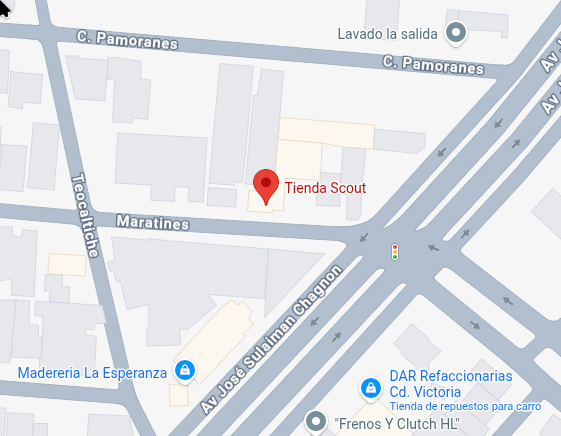
\includegraphics[width=0.7\textwidth]{img/figura_ubicacion_ccoe.png}
    \caption{Ubicación del CCoE de Honne en Ciudad Victoria, Tamaulipas.}
    \label{fig:ubicacion_ccoe}
\end{figure}

La Figura \ref{fig:organigrama} muestra la estructura organizacional de Honne. La Estadía se realizó dentro del equipo de Mesa de Servicio, ubicado en la columna de Servicios Administrados 2.0.

\begin{figure}[h]
    \centering
    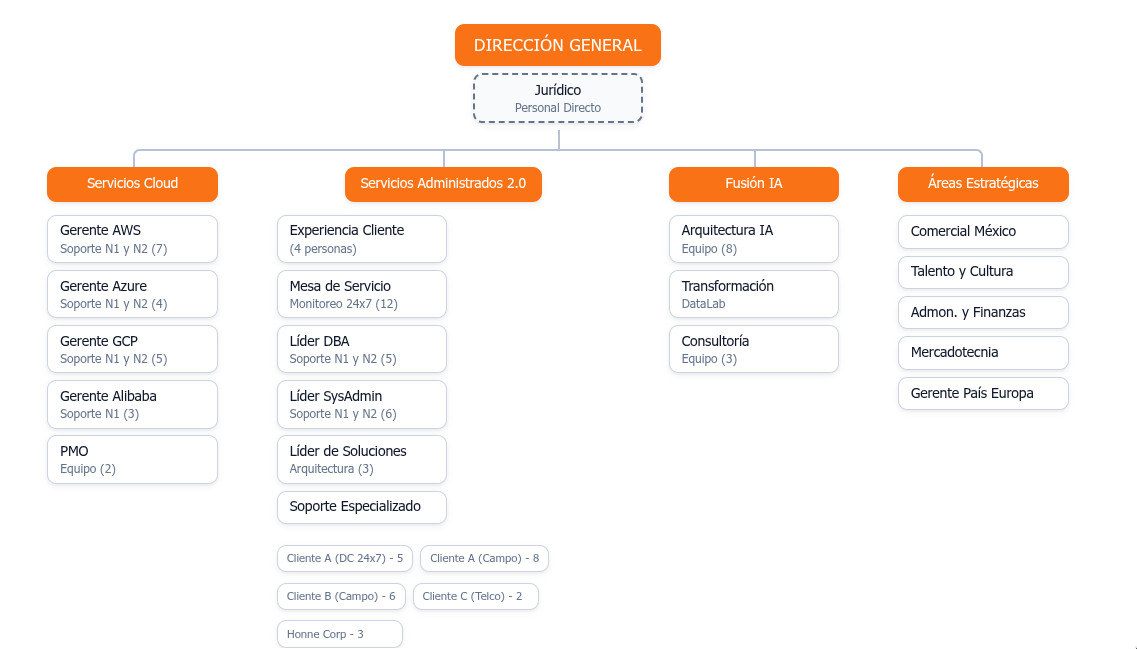
\includegraphics[width=0.8\textwidth]{img/figura_organigrama.png}
    \caption{Organigrama de Honne, con la Mesa de Servicio dentro de Servicios Administrados 2.0.}
    \label{fig:organigrama}
\end{figure}


\subsection{Descripción del área de trabajo y sus funciones}
\label{sec:area_trabajo}

El área en la que se realizó la Estadía es la Mesa de Servicio del CCoE. Su función principal es atender las solicitudes de los clientes relacionadas con sus instancias en la nube (AWS, Google Cloud Platform y Microsoft Azure), bases de datos y demás recursos de infraestructura, así como identificar errores o fallas en esas instancias y reportarlos a los usuarios para que soliciten su corrección.

La operación del área combina distintos canales y herramientas de trabajo. El correo electrónico de soporte técnico para el cliente es el canal principal para recibir alertas de errores e incidencias generadas por los distintos proveedores de cómputo en la nube. Además, para clientes específicos se emplean plataformas de monitoreo dedicadas como ServiceNow y TIBCO Scribe, mientras que Zendesk se utiliza principalmente para la gestión y asignación de tickets a las áreas responsables de la corrección de errores, como SysAdmin.

Los tickets atendidos abarcan una variedad de solicitudes de infraestructura y soporte, tales como la activación de autenticación multifactor (MFA), el restablecimiento de contraseñas, el ajuste de husos horarios, la validación de respaldos, la baja de usuarios, la asistencia en sesiones de trabajo y la elaboración de reportes periódicos de facturación, entre otros.

Como apoyo adicional, el área utiliza bots que automatizan parte del monitoreo, enviando notificaciones a través de Telegram sobre el estado de los servidores y la llegada de nuevos tickets en Zendesk.


\clearpage
\section{Planteamiento del problema}
\label{ch:planteamiento}

\subsection{Antecedentes del problema}
\label{sec:antecedentes_problema}

Como ya se describió en el apartado anterior, la Mesa de Servicio del CCoE manejaba varios frentes de trabajo de forma simultánea: monitoreo de correos, seguimiento de páginas de clientes específicos y gestión de tickets en Zendesk. A esta carga se sumaba un número considerable de alertas activas generadas en AWS que aún no habían sido verificadas, ya que el proceso para revisarlas no estaba asignado a una persona en específico.

\subsection{Definición del problema}
\label{sec:definicion_problema}

La saturación de la Mesa de Servicio se reflejaba de forma concreta en el número de alertas activas sin verificar: se llegaron a registrar 129 alertas generadas en AWS pendientes de revisión (ver Figura \ref{fig:alertas_aws}).

\begin{figure}[h]
    \centering
    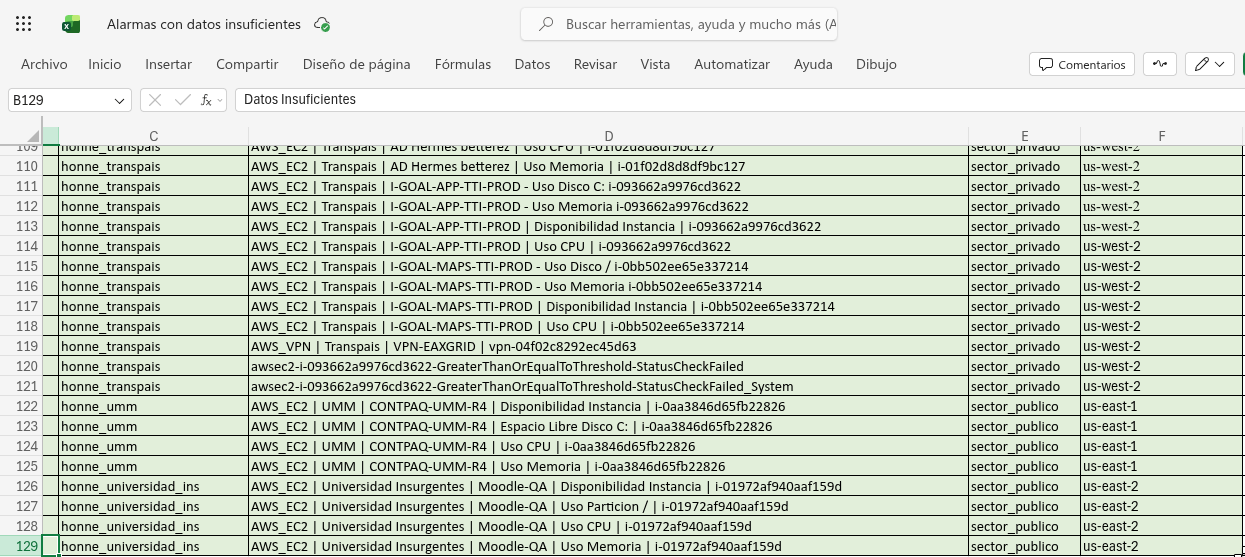
\includegraphics[width=0.8\textwidth]{img/figura_alertas_aws.png}
    \caption{Registro interno de alertas activas de AWS pendientes de verificación.}
    \label{fig:alertas_aws}
\end{figure}

Cada alerta debía revisarse manualmente para descartar falsos positivos, generados principalmente por dos causas: instancias que se apagaban de forma programada, lo cual generaba una alerta como si hubiera fallado aunque en realidad estaba funcionando como se esperaba; e instancias que ejecutaban tareas programadas, como respaldos, en horarios específicos, lo cual elevaba temporalmente el uso de CPU, disco, memoria o particiones hasta el 100\% y disparaba alertas de sobrecarga.

Aunque la verificación de alertas era responsabilidad de toda la Mesa de Servicio, no había una persona dedicada específicamente a esta tarea, por lo que las alertas reales y los falsos positivos se acumulaban en la misma bandeja, dificultando distinguir con rapidez cuáles requerían atención inmediata.

\subsection{Justificación}
\label{sec:justificacion}

Verificar cada alerta antes de reportarla era necesario porque Honne tiene la obligación contractual de informar a sus clientes sobre incidentes reales en sus instancias. Si un incidente real no se reportaba a tiempo, el cliente podía detectarlo por su cuenta y presentar una queja, lo cual representaba un riesgo de incumplimiento de contrato para la empresa. Al mismo tiempo, descartar los falsos positivos evitaba generar reportes innecesarios hacia clientes que no correspondían a una falla real.

Además, la incorporación de practicantes a esta tarea tenía como propósito liberar parte de la carga de trabajo de la Mesa de Servicio, distribuyendo la verificación de alertas para que el equipo pudiera enfocarse en la atención de incidentes reales y otras solicitudes.

\subsection{Objetivos}
\label{sec:objetivos}

\subsubsection{Objetivo general}
\label{subsec:objetivo_general}

Integrarse a la Mesa de Servicio del CCoE para apoyar en el uso de sus distintas herramientas de monitoreo y en el desarrollo de sus actividades diarias, contribuyendo a distribuir la carga de trabajo del área.

\subsubsection{Objetivos específicos}
\label{subsec:objetivos_especificos}

\begin{itemize}
    \item Verificar las alertas activas generadas en AWS, mediante las métricas de Amazon CloudWatch, para identificar falsos positivos y reportar los incidentes reales a los clientes correspondientes.
    \item Revisar los logs de instancias en Google Cloud Platform, mediante su consola de administración, para detectar problemas de latencia y errores recurrentes.
    \item Monitorear el estado de las soluciones y Agents de TIBCO Scribe (Scribesoft), revisando directamente los paneles de la plataforma, para verificar su disponibilidad.
    \item Desarrollar, en Python, un script de monitoreo automatizado que se conectara a TIBCO Scribe y notificara mediante un bot de Telegram cuando una solución presentara fallas recurrentes.
    \item Dar seguimiento a las alertas registradas en ServiceNow, mediante revisión constante de su bandeja, para notificar oportunamente al equipo responsable de su atención.
\end{itemize}

\subsection{Alcance y limitaciones}
\label{sec:alcance_limitaciones}

El apoyo brindado se centró en las herramientas de monitoreo utilizadas por la Mesa de Servicio del CCoE: alertas de AWS, logs de Google Cloud Platform, soluciones de TIBCO Scribe y alertas de ServiceNow, además del desarrollo de un script de automatización para una de ellas.

Como limitación, la función en todos los casos fue de detección y notificación, no de corrección directa de las fallas, ya que la resolución de incidentes correspondía a otras áreas, como SysAdmin. Tampoco se contó con un diagnóstico formal previo: las actividades fueron asignadas progresivamente por el asesor empresarial conforme surgían necesidades en el área.

\clearpage
\section{Capítulo 3 --- Marco teórico}
\label{ch:marcoteorico}
\textit{Incluir únicamente las metodologías, normas, software y conceptos técnicos que se usaron realmente (p. ej. DMAIC, PDCA, 5S, SMED, Lean, AMEF). Este capítulo debe fundamentar el método aplicado, no ser un tratado extenso.}


%\chapter{Metodología}
\clearpage
\section{Metodología}

Los métodos y herramientas utilizadas son la descripción detallada de las etapas
(o pasos, procedimiento) de desarrollo en que se dividió el proyecto y están
íntimamente relacionadas con los objetivos operativos. Se compara con una
receta de cocina, es decir, describir a detalle las actividades y acciones realizadas
en cada etapa de desarrollo, empleando un orden cronológico y en función de los
objetivos operativos. Sus características son:
\begin{itemize}
\item Descripción detallada de las etapas (o pasos) desarrolladas, las cuales están
relacionadas con cada objetivo operativos. Dependiendo del número de
objetivos, será el número de etapas de desarrollo reportadas.
\item En cada etapa de desarrollo, describir las herramientas académicas, técnicas
y computacionales que se utilizaron, indicando roles y responsabilidades.
Además, describir las asignaturas o aprendizajes que se obtuvieron durante tu
formación académica y fueron útiles en el proceso. Así mismo, describir
herramientas, equipos, tecnologías, etc., que se utilizaron durante el proyecto o
se aprendieron en la unidad económica.
\end{itemize}

\textit{El informe debe estar soportado por referencias, ademas incluir figuras y tablas. En los siguientes parrafos se ejemplifica como usar dichos elementos. }

De acuerdo con Ivan \cite{palos-sanchez_modelos_2019}, todos mienten, de la misma forma que Dr. House lo afirma de manera continua a lo largo de las 8 temporadas de la serie. 

Los sistemas de información constituyen un conjunto organizado de recursos —personas, datos, procesos y tecnología— que interactúan para recolectar, procesar, almacenar y distribuir información relevante dentro de una organización. Su propósito principal es apoyar la toma de decisiones, la coordinación y el control, así como facilitar el análisis y la visualización de información estratégica \cite{laudon2020, stair2018}. En el contexto actual, caracterizado por la digitalización y la globalización, los sistemas de información han evolucionado hacia plataformas integradas que permiten la gestión eficiente del conocimiento y la automatización de procesos empresariales \cite{turban2019}. Además, el uso de tecnologías emergentes como la inteligencia artificial y el análisis de datos ha ampliado sus capacidades, permitiendo generar valor a partir de grandes volúmenes de información \cite{davenport2018}.

Por otra parte, la implementación de sistemas de información implica retos importantes relacionados con la alineación estratégica, la seguridad de la información y la gestión del cambio organizacional. Es fundamental que estos sistemas estén alineados con los objetivos del negocio para maximizar su impacto y retorno de inversión \cite{ward2016}. Asimismo, la protección de datos y la ciberseguridad se han convertido en aspectos críticos debido al incremento de amenazas digitales \cite{whitman2018}. Finalmente, el éxito de un sistema de información depende en gran medida de la aceptación por parte de los usuarios y de una adecuada gestión del cambio, lo que requiere capacitación, comunicación efectiva y liderazgo organizacional \cite{heeks2006}.


En la figura \ref{fig:my_label}, se muestra una pantalla de una aplicación para contar las calorías de la comida mexicana. (Si la figura se mueve a la siguiente página, es NORMAL, no muevan nada!).
\begin{figure}[!tbh]
    \centering
    \includegraphics[width=0.5\linewidth]{img/calorias1.png}
    \caption{Aplicacion ``Mexican Food with Chilly'' \cite{Microsoft:Concepto}}
    \label{fig:my_label}
\end{figure}

En la tabla \ref{tab:my_label}, se muestra una tabla con el listado de los mejores futbolistas del mundo mundial. 

\begin{table}[!tbh]
    \centering
    \begin{tabular}{c|c} \hline
         Estudiante &  Nacionalidad \\ \hline
         Lionel Messi & Argentina  \\
         Cristiano Ronaldo & Portuguesa  \\
         Hector Hermoso Herrera & Mexicana \\ 
         \hline \hline
    \end{tabular}
    \caption{Otro ejemplo de tabla}
    \label{tab:my_label}
\end{table}


\clearpage
\section{Resultados}
\label{ch:resultados}

\subsection{Estado final}
\label{sec:estado_final}

Al cierre de la Estadía, las 129 alertas de AWS registradas en el diagnóstico inicial se clasificaron por completo entre patrones programados y fallas reales; ese trabajo tomó varios días de revisión continua.

El script de monitoreo de TIBCO Scribe también evolucionó respecto a la primera versión descrita en Metodología. En la versión final, la regla del estado de error fatal —que en un inicio se seguía revisando de forma manual— quedó automatizada: el script revisa el historial completo de cada solución, reporta cada ejecución en error fatal de forma individual sin repetir el mismo evento dos veces, y evita alertar sobre caídas que ya existían antes de que el script arrancara, para no saturar de avisos viejos. También se agregó la posibilidad de silenciar temporalmente, mediante un comando enviado al bot de Telegram, las alertas de una solución específica cuando el equipo ya tenía conocimiento de una falla en curso.

\subsection{Comparativo antes/después}
\label{sec:comparativo}

Antes de contar con el script, revisar a mano el estado de las soluciones de TIBCO Scribe tomaba entre 3 y 4 minutos por cada institución educativa: había que seleccionar cada solución en el menú, aplicar el filtro y esperar el resultado de la consulta, unas 16 veces por cliente. La ronda completa de las dos instituciones, es decir las 32 soluciones, tomaba entre 6 y 7 minutos, y se repetía cada 30 minutos durante toda la jornada. Con el script, esa misma ronda se hace sola cada 4 minutos y no ocupa el tiempo de nadie: el equipo únicamente atiende las notificaciones que el bot envía cuando encuentra una falla real.

\subsection{Evidencia fotográfica}
\label{sec:evidencia_fotografica}

\begin{figure}[h]
    \centering
    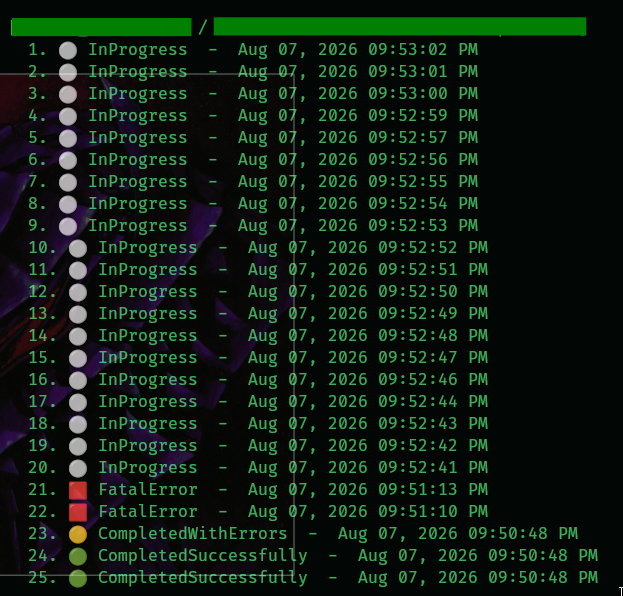
\includegraphics[width=0.8\textwidth]{img/figura_bot_estados.png}
    \caption{Los cuatro estados detectados por el bot de monitoreo de TIBCO Scribe.}
    \label{fig:bot_estados}
\end{figure}

\begin{figure}[h]
    \centering
    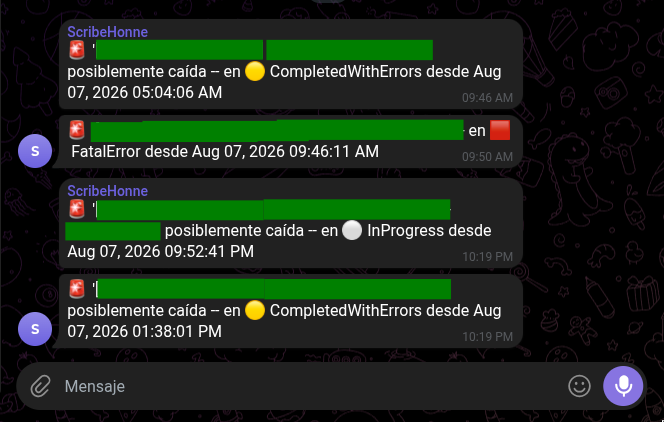
\includegraphics[width=0.8\textwidth]{img/figura_telegram_aviso.png}
    \caption{Avisos reales enviados por el bot al grupo de Telegram del equipo.}
    \label{fig:telegram_aviso}
\end{figure}

\subsection{Análisis de los resultados}
\label{sec:analisis_resultados}

El objetivo de automatizar el monitoreo de TIBCO Scribe se cumplió por completo: la versión final del script cubre incluso la regla del estado de error fatal, que en un inicio se seguía revisando de forma manual. Al dejar de hacerse cada 30 minutos de forma manual, el equipo pudo destinar ese tiempo a atender incidentes reales y otras tareas de monitoreo en lugar de revisiones repetitivas.

En el caso de AWS y Google Cloud Platform, el objetivo de verificar y reportar alertas también se cumplió, pero de forma manual en ambos casos; a diferencia de TIBCO Scribe, no se llegó a desarrollar una automatización similar para ellas, principalmente porque el tiempo de la Estadía se concentró en la herramienta que representaba la carga de trabajo más repetitiva. Para ServiceNow, esa automatización sí llegó a existir, pero fue obra de un compañero del equipo, no de este trabajo. Esa automatización pendiente para AWS y GCP queda como una oportunidad de mejora a futuro.


\clearpage
\section{Conclusiones y recomendaciones}
\label{ch:conclusiones}

\subsection{Cierre por objetivo específico}
\label{sec:cierre_objetivos}

\begin{itemize}
    \item \textbf{Verificar las alertas activas de AWS.} Se cumplió: las 129 alertas registradas en el diagnóstico inicial se clasificaron por completo entre patrones programados y fallas reales.
    \item \textbf{Revisar los logs de instancias en Google Cloud Platform.} Se cumplió, aplicando los criterios de más de 20 registros de error y el umbral de persistencia de latencia descritos en Metodología, de forma manual durante toda la Estadía.
    \item \textbf{Monitorear el estado de las soluciones y Agents de TIBCO Scribe.} Se cumplió, inicialmente de forma manual y después apoyado por el script de automatización.
    \item \textbf{Desarrollar un script de monitoreo automatizado para TIBCO Scribe.} Se cumplió y se superó lo planteado: la versión final del script automatizó incluso la regla del estado de error fatal, que en un inicio se pensaba mantener manual, y se agregó la posibilidad de silenciar alertas conocidas.
    \item \textbf{Dar seguimiento a las alertas de ServiceNow.} Se cumplió de forma manual y constante a lo largo de toda la Estadía, ya que esta herramienta no generaba notificaciones automáticas.
\end{itemize}

\subsection{Aprendizaje profesional y personal}
\label{sec:aprendizaje}

A nivel profesional, la Estadía me sirvió para entender mejor cómo funcionan los servicios en la nube y cómo viaja una petición entre un cliente y esos servicios. Sobre la automatización, lo que me quedó claro es que el problema de revisar la misma pantalla más de treinta veces seguidas no es únicamente el tiempo que consume: es que uno se cansa y empieza a pasar cosas por alto. El script no. También aprendí a distinguir una falla real de un falso positivo, un criterio que al principio tuve que consultar con el equipo, porque ellos ya lo aplicaban por experiencia, y que con las semanas terminé aplicando por mi cuenta.

A nivel personal, el mayor reto al inicio fue la comunicación con el personal del área: acostumbrarme a consultar dudas, coordinar tareas y reportar hallazgos con compañeros y superiores que ya tenían experiencia en el equipo. Con el tiempo esto dejó de ser un obstáculo. En cuanto al conocimiento técnico, llegué con las bases de AWS y salí con esas mismas bases más reforzadas por la práctica, ya que el trabajo en la Mesa de Servicio se concentró en el monitoreo con CloudWatch y no hubo oportunidad de profundizar en otras áreas de la plataforma. Lo que más me deja satisfecho de la Estadía es haber logrado que el script de monitoreo de TIBCO Scribe funcionara correctamente, al ser un desarrollo que hice por iniciativa propia.

\subsection{Recomendaciones a la empresa}
\label{sec:recomendaciones}

La principal recomendación es extender la automatización de monitoreo a las demás herramientas del área. El caso de TIBCO Scribe mostró que automatizar una revisión repetitiva libera tiempo del equipo para atender incidentes reales; aplicar un enfoque similar a la verificación de alertas de AWS, los logs de Google Cloud Platform y, sobre todo, a ServiceNow —donde actualmente no existe ningún tipo de notificación automática y se depende de la vigilancia constante del equipo— podría traer el mismo beneficio.

\subsection{Recomendaciones al programa académico}
\label{sec:recomendaciones_programa}

Se recomienda al programa académico reforzar contenidos prácticos relacionados con Google Cloud Platform y conceptos de monitoreo de infraestructura, ya que durante la Estadía este conocimiento tuvo que adquirirse directamente en campo. La formación académica sí incluyó una introducción a AWS, pero no cubrió otras plataformas de nube ni conceptos de monitoreo, más allá de la materia de Redes.

\subsection{Trabajo pendiente o siguiente fase}
\label{sec:trabajo_pendiente}

Como trabajo pendiente para una siguiente fase, se identifican dos líneas principales: extender la automatización desarrollada para TIBCO Scribe a las demás herramientas de monitoreo (AWS, Google Cloud Platform y ServiceNow), y migrar el script de monitoreo de TIBCO Scribe desde mi equipo de cómputo personal hacia un servidor o equipo de la empresa, para que continúe funcionando de forma permanente una vez concluida la Estadía.

La Estadía en \UnidadEconomica\ dejó dos cosas en la Mesa de Servicio del CCoE: las 129 alertas de AWS revisadas y clasificadas, y un script de monitoreo que funcionó durante el resto de la Estadía y que el equipo puede seguir usando si se migra a un equipo de la empresa. Para mí fue la primera experiencia de trabajo real en un área de TI: con horarios, con compañeros que dependían de lo que yo reportara y con clientes del otro lado.


%\clearpage
%\section*{Bibliografía}
%Agrega las referencias utilizadas.


\clearpage
%\Urlmuskip=0mu plus 1mu\relax
\addcontentsline{toc}{section}{Bibliografía} 
\printbibliography
 
\clearpage
\addcontentsline{toc}{section}{Anexos}
\section*{Anexos}

\subsection*{Cronograma de actividades}

\begin{itemize}
    \item \textbf{Primer mes (mediados de mayo -- mediados de junio):} verificación de alertas activas de AWS.
    \item \textbf{Segundo mes (mediados de junio -- mediados de julio):} revisión de logs de instancias en Google Cloud Platform.
    \item \textbf{Tercer mes en adelante (mediados de julio -- cierre de la Estadía):} monitoreo de TIBCO Scribe y desarrollo del script de automatización.
    \item \textbf{Constante durante toda la Estadía:} seguimiento a las alertas de ServiceNow.
\end{itemize}

\subsection*{Código fuente del script de monitoreo}

A continuación se incluye el código completo del script de monitoreo de TIBCO Scribe desarrollado durante la Estadía, descrito en Metodología.

\lstinputlisting[caption={Script completo de monitoreo de TIBCO Scribe.}, label={lst:monitoreo_completo}]{monitoreo.py}

\clearpage
\thispagestyle{fancy}
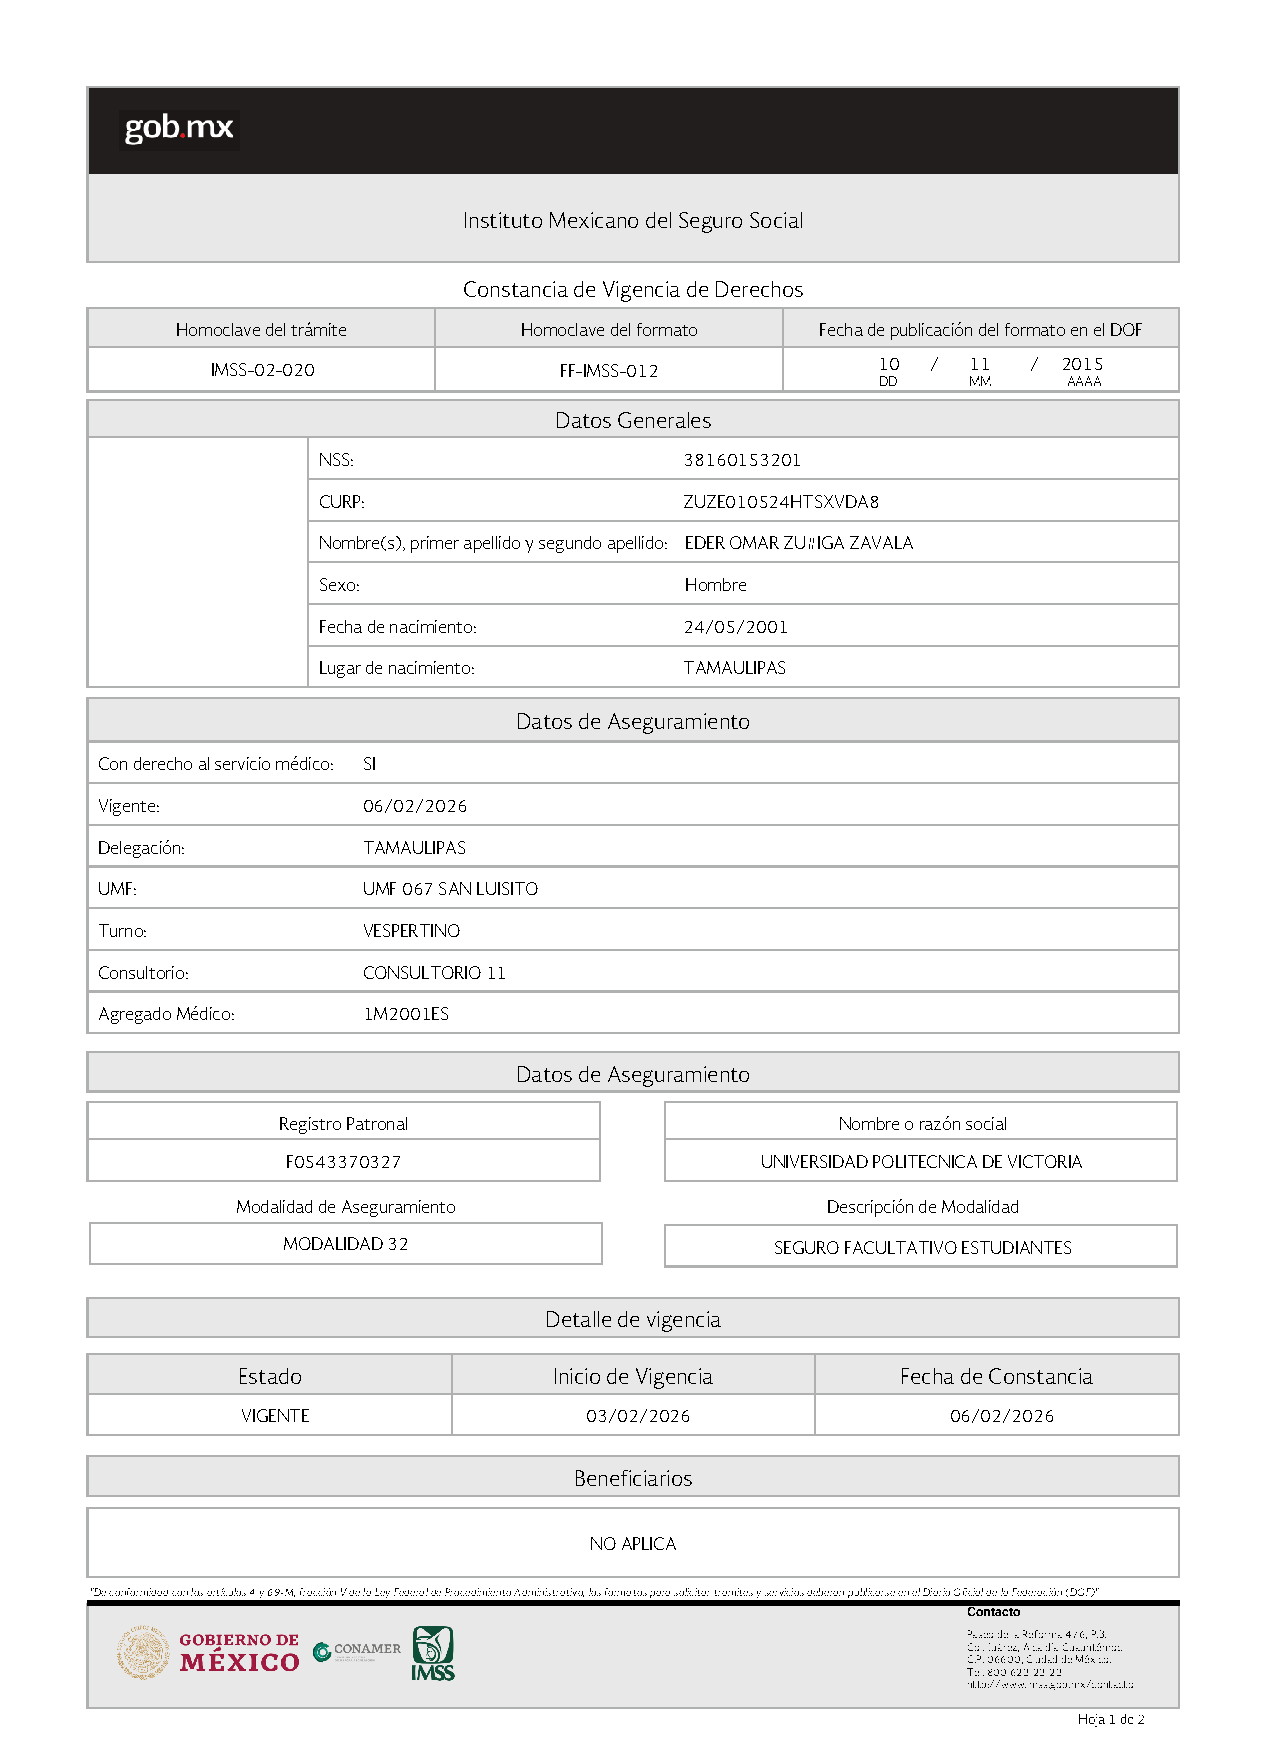
\includepdf[pages={1}]{documentosDigitalizados/SeguroFacultativo.pdf}

% En las siguientes 2 paginas, debe incluir una digitalización de calidad de sus respectivas cartas, no una fotografia toda cucha tomada con su celular de Coppel
% Pagina 1: Digitalización de la carta de presentación (sustituir por una original en el empastado)
\clearpage
\thispagestyle{fancy}
%\pagenumbering{roman}
%\setcounter{page}{1}

\includepdf[pages={1}]{documentosDigitalizados/CartaPresentacion.pdf}

% Pagina 2: Digitalización de la carta de aceptación (sustituir por una original en el empastado)
\clearpage
\thispagestyle{fancy}

\includepdf[pages={1}]{documentosDigitalizados/CartaAceptacion.pdf}

% Pagina 3: Digitalización de la carta de liberación (PENDIENTE: aún no existe el documento)
% Cuando esté disponible, guardarla en documentosDigitalizados/CartaLiberacion.pdf y descomentar:
% \clearpage
% \thispagestyle{fancy}
% 
\includepdf[pages={1}]{documentosDigitalizados/CartaLiberacion.pdf}

%\chapter*{Rúbrica para la Evaluación del Reporte de Estadía}
\clearpage
%\section*{Rúbrica para la Evaluación del Reporte de Estadía}
\newcommand{\SizeFont}{\footnotesize}

\begin{center}
\large {\textbf{Rúbrica para la Evaluación del Reporte de Estadía}}

\begin{sidewaystable}
\begin{longtable}{|p{0.5cm}|p{13cm}|p{1.5cm}|p{3cm}|}
\hline
%Fecha y lugar en que se emite: \textbf{Ciudad Victoria, Tamaulipas, a \fechaAutorizacionInforme } \\[0.125cm]
\multicolumn{4}{|l|}{Nombre completo del estudiante: \textbf{\NombreAlumno} }\\
\multicolumn{4}{|l|}{Matrícula:  \textbf{\Matricula}}  \\
\multicolumn{4}{|l|}{PERIODO: \ncuatrimestre } \\
\multicolumn{4}{|l|}{Nombre del evaluador: \nasesorinstitucional} \\
\multicolumn{4}{|l|}{ } \\
\multicolumn{4}{|l|}{Firma del Evaluador: \_\_\_\_\_\_\_\_\_\_\_\_\_\_\_\_\_\_\_\_\_\_\_\_  }\\
\multicolumn{4}{|l|}{Calificación Final: \_\_\_ / 100} \\ \hline
Valor & Características a cumplir & Puntos & Observaciones \\ \hline
\SizeFont 6 & \SizeFont Resumen ejecutivo y abstract: Indica qué se realizó, cómo se realizó y qué se obtuvo. (una cuartilla en español e inglés) & & \\ \hline
\SizeFont 6 & \SizeFont Contenido temático: Describe correctamente el contenido del documento & & \\ \hline
\SizeFont 6 & \SizeFont Introducción: El informe cumple con introducir al lector de una manera atractiva el panorama general del trabajo realizado en la unidad económica.  & & \\ \hline
\SizeFont 6 & \SizeFont Descripción de la unidad económica: Se redactan los detalles de los antecedentes del departamento, la empresa, giro, misión, visión, infraestructura, ubicación. & & \\\hline
\SizeFont 6 & \SizeFont Objetivos operativos: Describen las acciones a cumplir mediante actividades establecidas por el asesor empresarial & & \\ \hline
\SizeFont 24 & \SizeFont Metodología: Descripción a detalle de las etapas y procedimientos utilizados en el proyecto & & \\ \hline
\SizeFont 18 & \SizeFont Resultados: Interpreta y analiza los resultados obtenidos durante su estadía. & & \\ \hline
\SizeFont 12 & \SizeFont Conclusiones: Las conclusiones son claras y acordes con el objetivo esperado & & \\ \hline
\SizeFont 6 & \SizeFont Bibliografía y anexos: Cita correctamente las fuentes de información utilizando un estilo de referencia; anexa cartas correspondientes & & \\ \hline
\SizeFont 10 & \SizeFont Responsabilidad: Entregó el reporte en la fecha y hora señalada. Asistió al menos al 80\% de sus días de Estadía & & \\ \hline
\end{longtable}
\end{sidewaystable}

\end{center}

%\chapter*{Rúbrica para Exposición}
\clearpage
\begin{center}
\large {\textbf{Rúbrica para Exposición del Reporte de Estadía}}
\end{center}


\begin{longtable}{|p{3.75cm}|p{3.75cm}|p{3.75cm}|p{3.75cm}|}
\hline
 & \multicolumn{3}{c|}{Nivel de logro} \\ \hline
%A &B  & C & D \\
Criterio &  Bueno ( 10\% ) & Regular (7\% ) & Menor a lo esperado (5\%) \\ \hline
\SizeFont Dominio del tema (10\%) & \SizeFont Utiliza todos los términos y conceptos de manera correcta. & \SizeFont Utiliza la mayoría términos y conceptos de manera correcta & \SizeFont Confunde los términos y conceptos. \\ \hline

\SizeFont  Presentación de material visual (10\%) & \SizeFont Las  diapositivas usadas tienen fondo claro, letras, tablas e imágenes visibles. La presentación contiene los aspectos relevantes de la Estadía
& \SizeFont Las  diapositivas usadas presentan dificultad para su apreciación visual. La presentación contiene los aspectos relevantes de la Estadía & \SizeFont Las  diapositivas usadas presentan dificultad para su apreciación visual. La presentación carece de algunos aspectos relevantes de la Estadía. \\ \hline

\SizeFont   Comunicación y expresión (10\%)  & \SizeFont   Su volumen de voz es comprensible. Su expresión corporal manifiesta seguridad ejecutiva. Su atuendo cumple los estándares de ser formal o semiformal.  Mantiene una línea de respeto en general. &  \SizeFont   Su volumen de voz no es comprensible. Su expresión corporal manifiesta inseguridad. Su atuendo cumple los estándares de ser formal o semiformal.  Mantiene una línea de respeto en general. &
\SizeFont  Su volumen de voz no es comprensible. Su expresión corporal manifiesta inseguridad. Su atuendo no cumple los estándares de ser formal o semiformal.  Realiza alguna falta de respeto. \\ \hline

\SizeFont   Respuestas (10\%) & \SizeFont Las respuestas son consistentes y con parámetros de lógica operativa. & \SizeFont    Las respuestas no son consistentes pero tienen parámetros de lógica operativa. & \SizeFont    Las respuestas son difusas e incoherentes.  \\ \hline


\multicolumn{2}{|c|}{\textbf{Ponderación final de su exposición:}} & \multicolumn{2}{c|}{\_\_\_ /100} \\ \hline
%\multicolumn{2}{|c|}{Día / Mes / Año} &  \multicolumn{2}{c|}{\_\_\_\_ / \_\_\_\_\_\_\_\_ / \_\_\_\_  } \\  \hline
\multicolumn{2}{|c|}{Día / Mes / Año} &  \multicolumn{2}{c|}{\DiaEvaluacionPesentacion / \MesEvaluacionPesentacion / \AnhoEvaluacionPesentacion} \\  \hline
\multicolumn{2}{|c}{ }& \multicolumn{2}{|c|}{ }  \\
\multicolumn{2}{|c}{ }& \multicolumn{2}{|c|}{ }  \\    
\multicolumn{2}{|c}{Comentario adicional} & \multicolumn{2}{|c|}{ } \\  
\multicolumn{2}{|c}{ }& \multicolumn{2}{|c|}{ }  \\  
\multicolumn{2}{|c}{ }& \multicolumn{2}{|c|}{ }  \\  \hline



\end{longtable}

\end{document}
